\documentclass[12pt,a4paper]{article}
\usepackage[utf8]{vietnam}
\usepackage{amsmath,amssymb}
\usepackage{geometry}
\geometry{top=1.5cm,bottom=1.2cm,left=1.4cm,right=1.4cm,headheight=28pt,headsep=12pt,footskip=18pt}
\usepackage{tikz}
\usepackage{xcolor}
\usepackage{enumerate}
\usepackage{graphicx}
\usepackage[version=4]{mhchem}
\usepackage{fancyhdr}
\usepackage{ex_test}

\renewcommand{\baselinestretch}{0.96}
\setlength{\parskip}{0pt}

\definecolor{hfRed}{RGB}{211,47,47}
\definecolor{hfGreen}{RGB}{139,195,144}

\pagestyle{fancy}
\fancyhf{}
\fancyhead[L]{\small\itshape\color{hfRed} Tài liệu lưu hành nội bộ}
\fancyhead[R]{\small\itshape\color{hfRed} Thầy \textbf{TRẦN VĂN THẠNH} - 0777.470.803}
\renewcommand{\headrulewidth}{0.8pt}
\renewcommand{\headrule}{\hbox to\headwidth{\color{hfGreen}\leaders\hrule height \headrulewidth\hfill}}

\fancyfoot[L]{\small\itshape\color{hfRed} CS1: 6/15 Nguyễn Hoàng, P. Kim Long, TP Huế \quad|\quad CS2: 24 Đặng Thái Thân, TP Huế}
\fancyfoot[R]{\small\bfseries\color{hfRed} Trang \thepage}
\renewcommand{\footrulewidth}{0.8pt}
\renewcommand{\footrule}{\hbox to\headwidth{\color{hfGreen}\leaders\hrule height \footrulewidth\hfill}}

\fancypagestyle{firstpage}{
  \fancyhf{}
  \renewcommand{\headrulewidth}{0pt}
  \fancyfoot[L]{\small\itshape\color{hfRed} CS1: 6/15 Nguyễn Hoàng, P. Kim Long, TP Huế \quad|\quad CS2: 24 Đặng Thái Thân, TP Huế}
  \fancyfoot[R]{\small\bfseries\color{hfRed} Trang \thepage}
  \renewcommand{\footrulewidth}{0.8pt}
  \renewcommand{\footrule}{\hbox to\headwidth{\color{hfGreen}\leaders\hrule height \footrulewidth\hfill}}
}

\begin{document}
\thispagestyle{firstpage}

\noindent
\begin{minipage}[t]{0.44\textwidth}
	\centering\fontsize{10pt}{12pt}\selectfont
	\textbf{SỞ GIÁO DỤC VÀ ĐÀO TẠO THỪA THIÊN HUẾ}\\
	\textbf{TRƯỜNG THPT CHUYÊN QUỐC HỌC}\\
	\textbf{ĐỀ CHÍNH THỨC}\\
	\textit{(Đề thi có 04 trang)}
\end{minipage}\hfill
\begin{minipage}[t]{0.54\textwidth}
	\centering\small
	\textbf{ĐỀ KIỂM TRA ĐỊNH KỲ CHƯƠNG 1 (ESTER -- LIPID)}\\
	\textbf{MÔN: HOÁ HỌC -- LỚP 12}\\
	\textit{Thời gian làm bài: 50 phút (không kể thời gian phát đề)}\\
	\fbox{\textbf{MÃ ĐỀ: 101}}
\end{minipage}

\smallskip
\noindent\hrulefill
\smallskip

\noindent\textbf{Họ, tên thí sinh:} \dotfill\ \textbf{Lớp:} \dotfill\ \textbf{Số báo danh:} \dotfill

\smallskip
\noindent\textit{(Cho biết nguyên tử khối: H = 1; C = 12; N = 14; O = 16; Na = 23; K = 39; Br = 80).}
\smallskip

\noindent
\textbf{PHẦN I (4,5 điểm -- 18 câu): Câu trắc nghiệm nhiều phương án lựa chọn.}\\
\textit{Thí sinh trả lời từ câu 1 đến câu 18. Mỗi câu hỏi thí sinh chỉ chọn một phương án.}

\Opensolutionfile{ans}[ans-de01hs]

\begin{ex}
Chất nào sau đây thuộc loại ester?
\choice
{$\ce{CH3COOC2H5}$}
{$\ce{HOOCCH3}$}
{$\ce{H2N-CH2-COOH}$}
{$\ce{CH3CHO}$}
\loigiai{}
\end{ex}

\begin{ex}
Phản ứng điều chế xà phòng từ chất béo được gọi là phản ứng
\choice
{ester hóa}
{xà phòng hóa}
{trung hòa}
{hydrate hóa}
\loigiai{}
\end{ex}

\begin{ex}
Dầu chuối là ester có tên isoamyl acetate, được điều chế từ
\choice
{$\ce{CH3OH}$, $\ce{CH3COOH}$}
{$\ce{(CH3)2CH-CH2OH}$, $\ce{CH3COOH}$}
{$\ce{C2H5COOH}$, $\ce{C2H5OH}$}
{$\ce{CH3COOH}$, $\ce{(CH3)2CH-CH2-CH2OH}$}
\loigiai{}
\end{ex}

\begin{ex}
Một số ester được dùng trong hương liệu, mĩ phẩm, bột giặt là nhờ các ester
\choice
{là chất lỏng dễ bay hơi}
{có mùi thơm, an toàn với người}
{có thể bay hơi nhanh sau khi sử dụng}
{đều có nguồn gốc từ thiên nhiên}
\loigiai{}
\end{ex}

\begin{ex}
Thủy phân ester nào sau đây trong dung dịch $\ce{NaOH}$ thu được sodium formate?
\choice
{$\ce{CH3COOCH3}$}
{$\ce{CH3COOC2H5}$}
{$\ce{HCOOC2H5}$}
{$\ce{CH3COOC3H7}$}
\loigiai{}
\end{ex}

\begin{ex}
Số đồng phân ester ứng với công thức phân tử $\ce{C4H8O2}$ là
\choice
{2}
{3}
{4}
{5}
\loigiai{}
\end{ex}

\begin{ex}
Công thức của tristearin là
\choice
{$\ce{(C2H5COO)3C3H5}$}
{$\ce{(C17H35COO)3C3H5}$}
{$\ce{(CH3COO)3C3H5}$}
{$\ce{(HCOO)3C3H5}$}
\loigiai{}
\end{ex}

\begin{ex}
Thực hiện phản ứng ester hoá giữa $\ce{HOOC-COOH}$ với hỗn hợp $\ce{CH3OH}$ và $\ce{C2H5OH}$ thu được tối đa bao nhiêu ester hai chức?
\choice
{2}
{3}
{1}
{4}
\loigiai{}
\end{ex}

\begin{ex}
Công thức phân tử của oleic acid là
\choice
{$\ce{C2H5COOH}$}
{$\ce{HCOOOH}$}
{$\ce{CH3COOH}$}
{$\ce{C17H33COOH}$}
\loigiai{}
\end{ex}

\begin{ex}
Công thức của triolein là
\choice
{$\ce{(C17H33COO)3C3H5}$}
{$\ce{(HCOO)3C3H5}$}
{$\ce{(C2H5COO)3C3H5}$}
{$\ce{(CH3COO)3C3H5}$}
\loigiai{}
\end{ex}

\begin{ex}
Cho các chất sau: (1) alcohol ethylic, (2) acetic acid, (3) nước, (4) methyl formate. Thứ tự nhiệt độ sôi giảm dần là
\choice
{(1) $>$ (4) $>$ (3) $>$ (2)}
{(1) $>$ (2) $>$ (3) $>$ (4)}
{(1) $>$ (3) $>$ (2) $>$ (4)}
{(2) $>$ (3) $>$ (1) $>$ (4)}
\loigiai{}
\end{ex}

\begin{ex}
Xà phòng và chất giặt rửa có đặc điểm chung nào sau đây?
\choice
{Không tan trong nước}
{Là muối sodium hoặc potassium của acid béo}
{Là muối sulfonate hoặc sulfate của acid béo}
{Thường có cấu tạo gồm hai phần là phần không phân cực (kị nước) và phần phân cực (ưa nước)}
\loigiai{}
\end{ex}

\begin{ex}
Cho các chất sau: $\ce{CH3[CH2]7CH=CH[CH2]7COONa}$, $\ce{CH3[CH2]14COOK}$, $\ce{CH3[CH2]10COOK}$ và $\ce{CH3COONa}$. Trong các chất nêu trên, có bao nhiêu chất có thể là thành phần chính của xà phòng?
\choice
{1}
{2}
{3}
{4}
\loigiai{}
\end{ex}

\begin{ex}
Phát biểu nào sau đây về xà phòng là đúng?
\choice
{Xà phòng có thành phần chính là muối sodium hoặc potassium của carboxylic acid}
{Các phân tử xà phòng đều có đầu kị nước gắn với đuôi dài ưa nước}
{Xà phòng mất tính giặt rửa khi sử dụng với nước cứng}
{Nhược điểm của xà phòng là khó bị phân huỷ hoặc phân huỷ chậm, do đó gây hại cho hệ sinh thái}
\loigiai{}
\end{ex}

\begin{ex}
Trong số các vật phẩm tiêu dùng sau: xà phòng bánh, dầu gội đầu, nước bồ kết và baking soda ($\ce{NaHCO3}$), số vật phẩm có thành phần chất giặt rửa tự nhiên và tổng hợp là
\choice
{1}
{2}
{3}
{4}
\loigiai{}
\end{ex}

\begin{ex}
Loại dầu nào sau đây không phải là chất béo?
\choice
{dầu vừng}
{dầu oliu}
{dầu gan cá}
{dầu luyn}
\loigiai{}
\end{ex}

\begin{ex}
Cho các phản ứng sau:\\
(1) Thuỷ phân ester trong môi trường acid.\\
(2) Thuỷ phân ester trong dung dịch $\ce{NaOH}$, đun nóng.\\
(3) Cho ester tác dụng với dung dịch $\ce{KOH}$, đun nóng.\\
(4) Thuỷ phân dẫn xuất halogen trong dung dịch $\ce{NaOH}$, đun nóng.\\
(5) Cho carboxylic acid tác dụng với dung dịch $\ce{NaOH}$.\\
Những phản ứng nào không được gọi là phản ứng xà phòng hoá?
\choice
{(1), (2), (3), (4)}
{(1), (4), (5)}
{(1), (3), (4), (5)}
{(3), (4), (5)}
\loigiai{}
\end{ex}

\begin{ex}
Đun nóng acid acetic với isoamyl alcohol $\ce{(CH3)2CH-CH2CH2OH}$ có $\ce{H2SO4}$ đặc xúc tác thu được isoamyl acetate (dầu chuối). Tính lượng dầu chuối thu được từ $132{,}35\text{ gam}$ acid acetic đun nóng với $200\text{ gam}$ isoamyl alcohol (biết hiệu suất phản ứng đạt 68\%).
\choice
{$97{,}5\text{ gam}$}
{$195{,}0\text{ gam}$}
{$292{,}5\text{ gam}$}
{$159{,}0\text{ gam}$}
\loigiai{}
\end{ex}

\Closesolutionfile{ans}

\vspace{0.3cm}
\noindent
\textbf{PHẦN II (4,0 điểm -- 4 câu): Câu trắc nghiệm đúng sai.}\\
\textit{Thí sinh trả lời từ câu 1 đến câu 4. Trong mỗi ý a), b), c), d) ở mỗi câu, thí sinh chọn đúng hoặc sai.}

\setcounter{ex}{0}

\begin{ex}
Cho các triglyceride X, Y với công thức cấu tạo sau:
\begin{center}
	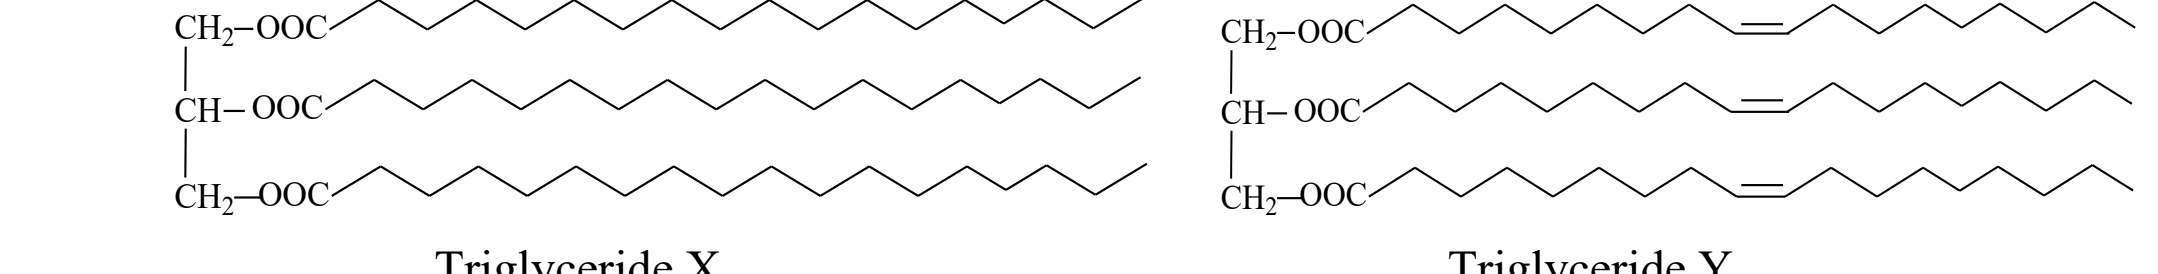
\includegraphics[width=14cm]{images_crop_de01/triglyceride_XY.png}
\end{center}
Em hãy cho biết các phát biểu sau đây là đúng hay sai:
\choiceTF[t]
{Triglyceride X có tên gọi là tripalmitin.}
{X là chất béo no, Y là chất béo không no.}
{X, Y đều tan tốt trong nước.}
{Hydrogen hoá Y thu được X.}
\loigiai{}
\end{ex}

\begin{ex}
Nhiệt độ sôi và độ tan của một số ester, carboxylic acid và alcohol có cùng số nguyên tử carbon được cho trong bảng sau:
\begin{center}
\begin{tabular}{|l|c|c|}
\hline
\textbf{Công thức} & \textbf{Nhiệt độ sôi ($^\circ\text{C}$)} & \textbf{Độ tan ở 25 $^\circ\text{C}$ (g/100 g nước)} \\ \hline
$\ce{HCOOCH3}$ & $31{,}5$ & $23{,}0$ \\ \hline
$\ce{HCOOC2H5}$ & $54{,}2$ & $12{,}0$ \\ \hline
$\ce{CH3COOH}$ & $117{,}9$ & Tan vô hạn \\ \hline
$\ce{C2H5COOH}$ & $141{,}0$ & Tan vô hạn \\ \hline
$\ce{C2H5OH}$ & $78{,}4$ & Tan vô hạn \\ \hline
$\ce{CH3CH2CH2OH}$ & $97{,}2$ & Tan vô hạn \\ \hline
\end{tabular}
\end{center}
Em hãy cho biết các phát biểu sau đây là đúng hay sai:
\choiceTF[t]
{Do không tạo được liên kết hydrogen giữa các phân tử nên ester có nhiệt độ sôi thấp hơn nhiệt độ sôi của carboxylic acid và alcohol có cùng số nguyên tử carbon.}
{Do có khả năng tạo liên kết hydrogen yếu với nước nên ester thường ít tan trong nước hơn so với carboxylic acid và alcohol có cùng số carbon.}
{Carboxylic acid có nhiệt độ sôi cao hơn alcohol có cùng số nguyên tử carbon.}
{Methanol có khả năng tan vô hạn trong nước.}
\loigiai{}
\end{ex}

\begin{ex}
Các phát biểu sau đây về xà phòng và chất giặt rửa là đúng hay sai?
\choiceTF[t]
{Xà phòng và chất giặt rửa thường có cấu tạo gồm hai phần: ưa nước và kị nước.}
{Xà phòng hoá tripalmitin với dung dịch $\ce{NaOH}$ thu được sản phẩm là $\ce{C15H29COONa}$ và glycerol.}
{Chất giặt rửa tổng hợp thường được điều chế từ chất béo.}
{Mỡ động vật, dầu thực vật là nguyên liệu để sản xuất xà phòng.}
\loigiai{}
\end{ex}

\begin{ex}
Các phát biểu sau đây là đúng hay sai?
\choiceTF[t]
{Chất giặt rửa thường là muối sodium alkylsulfate hoặc alkylbenzene sulfonate.}
{Phân tử chất giặt rửa gồm một đầu kị nước gắn với một đầu ưa nước.}
{Khi giặt rửa bằng nước cứng nên sử dụng xà phòng.}
{Phản ứng thuỷ phân chất béo trong môi trường kiềm ($\ce{NaOH, KOH}$) thuộc loại phản ứng xà phòng hoá.}
\loigiai{}
\end{ex}

\vspace{0.3cm}
\noindent
\textbf{PHẦN III (1,5 điểm -- 6 câu): Câu trắc nghiệm yêu cầu trả lời ngắn.}\\
\textit{Thí sinh trả lời từ câu 1 đến câu 6. Mỗi câu hỏi thí sinh điền câu trả lời ngắn gọn theo yêu cầu.}

\setcounter{ex}{0}

\begin{ex}
Khi xà phòng hóa triglyceride X bằng dung dịch $\ce{NaOH}$ dư, đun nóng, thu được sản phẩm gồm glycerol, sodium oleate, sodium stearate và sodium palmitate. Số đồng phân cấu tạo thỏa mãn tính chất trên của X là bao nhiêu?
\loigiai{}
\end{ex}

\begin{ex}
Cho triolein lần lượt vào mỗi ống nghiệm chứa riêng biệt: $\ce{Na}$, $\ce{Cu(OH)2}$, $\ce{CH3OH}$, dung dịch $\ce{Br2}$, dung dịch $\ce{NaOH}$. Trong điều kiện thích hợp, số phản ứng xảy ra là bao nhiêu?
\loigiai{}
\end{ex}

\begin{ex}
Một loại chất béo có chứa 80\% tristearin về khối lượng. Để sản xuất ba nghìn (3000) bánh xà phòng cần dùng tối thiểu $x\text{ kg}$ loại chất béo trên cho phản ứng với dung dịch $\ce{NaOH}$, đun nóng. Biết hiệu suất phản ứng đạt 90\%. Biết rằng trong mỗi bánh xà phòng có chứa $60\text{ gam}$ sodium stearate. Giá trị của $x$ là bao nhiêu? \textit{(Làm tròn kết quả đến một chữ số thập phân).}
\begin{flushright}
	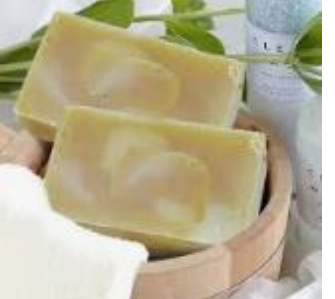
\includegraphics[width=3.5cm]{images_crop_de01/soap_bar.png}
\end{flushright}
\loigiai{}
\end{ex}

\begin{ex}
Cho $0{,}1\text{ mol}$ butanoic acid tác dụng với $0{,}1\text{ mol}$ methyl alcohol có mặt $\ce{H2SO4}$ đặc làm xúc tác. Tính khối lượng ester tạo thành theo gam, biết 67\% alcohol chuyển hoá thành ester. \textit{(Làm tròn kết quả đến hai chữ số thập phân).}
\loigiai{}
\end{ex}

\begin{ex}
Một loại dầu thực vật trong đó thành phần chất béo chứa hai gốc linoleate, một gốc oleate và thành phần phần trăm khối lượng chất béo trong dầu thực vật là 88\%. Tính chỉ số ester của dầu thực vật đó. (Biết chỉ số ester là số miligam $\ce{KOH}$ dùng để xà phòng hoá hết lượng triglyceride có trong 1 g chất béo).
\loigiai{}
\end{ex}

\begin{ex}
Số miligam $\ce{KOH}$ dùng để xà phòng hoá hết lượng triglyceride có trong 1 g chất béo được gọi là chỉ số ester hoá của loại chất béo đó. Tính chỉ số ester của một loại chất béo chứa 65\% tristearin và 23\% triolein (còn lại là tạp chất không phản ứng). \textit{(Kết quả làm tròn đến phần nguyên).}
\loigiai{}
\end{ex}

\begin{center}
\textbf{--------- HẾT ---------}
\end{center}

\end{document}
